% Autor: Leonhard Segger, Alexander Neuwirth
% Datum: 2017-10-30
\documentclass[
	% Papierformat
	a4paper,
	% Schriftgröße (beliebige Größen mit „fontsize=Xpt“)
	12pt,
	% Schreibt die Papiergröße korrekt ins Ausgabedokument
	pagesize,
	% Sprache für z.B. Babel
	ngerman
]{scrartcl}

% Achtung: Die Reihenfolge der Pakete kann (leider) wichtig sein!
% Insbesondere sollten (so wie hier) babel, fontenc und inputenc (in dieser
% Reihenfolge) als Erstes und hyperref und cleveref (Reihenfolge auch hier
% beachten) als Letztes geladen werden!

\usepackage{tikz}
\usetikzlibrary{calc,patterns,angles,quotes} % loads some tikz extensions\usepackage{tikz}
\usetikzlibrary{babel}

% Silbentrennung etc.; Sprache wird durch Option bei \documentclass festgelegt
\usepackage{babel}
% Verwendung der Zeichentabelle T1 (Sonderzeichen etc.)
\usepackage[T1]{fontenc}
% Legt die Zeichenkodierung der Eingabedatei fest, z.B. UTF-8
\usepackage[utf8]{inputenc}
% Schriftart
\usepackage{lmodern}
% Zusätzliche Sonderzeichen
\usepackage{textcomp}

% Mathepaket (intlimits: Grenzen über/unter Integralzeichen)
\usepackage[intlimits]{amsmath}
% Ermöglicht die Nutzung von \SI{Zahl}{Einheit} u.a.
\usepackage{siunitx}
% Zum flexiblen Einbinden von Grafiken (\includegraphics)
\usepackage{graphicx}
% Abbildungen im Fließtext
\usepackage{wrapfig}
% Abbildungen nebeneinander (subfigure, subtable)
\usepackage{subcaption}
% Funktionen für Anführungszeichen
\usepackage{csquotes}
\MakeOuterQuote{"}
% Zitieren, Bibliografie
\usepackage[sorting=none]{biblatex}


% Zur Darstellung von Webadressen
\usepackage{url}
%chemische Formeln
\usepackage[version=4]{mhchem}
% siunitx: Deutsche Ausgabe, Messfehler getrennt mit ± ausgeben
\usepackage{floatrow}
\floatsetup[table]{capposition=top}
\usepackage{float}
% Verlinkt Textstellen im PDF-Dokument
\usepackage[unicode]{hyperref}
% "Schlaue" Referenzen (nach hyperref laden!)
\usepackage{cleveref}
\sisetup{
	locale=DE,
	separate-uncertainty
}
\bibliography{BA-C-04_MI_19-11-2018_References}

\begin{document}

	\begin{titlepage}
		\centering
		{\scshape\LARGE Versuchsbericht zu \par}
		\vspace{1cm}
		{\scshape\huge MI - Michelson-Interferometer \par} %TODO fine?
		\vspace{2.5cm}
		{\LARGE Gruppe BA-C-04 \par}
		\vspace{0.5cm}

		{\large Alexander Neuwirth (E-Mail: a\_neuw01@wwu.de) \par}
		{\large Leonhard Segger (E-Mail: l\_segg03@uni-muenster.de) \par}
		\vfill

		durchgeführt am 19.11.2018\par
		betreut von\par
		{\large Victor Kärcher} %TODO Anpassen

		\vfill

		{\large \today\par}
	\end{titlepage}
	\tableofcontents
	\newpage

	%TODO mehr TODO in Default

	\section{Kurzfassung}
	% Hypothese	und deren Ergebnis, wenn Hypothese ist, dass nur Theorie erfüllt, sagen: Erwartung: Theorie aus einführung (mit reflink) erfüllt
	% Ergebnisse, auch Zahlen, mindestens wenn's halbwegs Sinn ergibt
	% Was wurde gemacht
	% manche leute wollen Passiv oder "man", manche nicht
	\section{Theorie}

	\subsection{Brechungsindex Bestimmung von Glas durch Rotation}
	In \cref{fig_glass_rotation} ist der Strahlengang für einen Einfallswinkel von $\alpha=0$ und $\alpha>0$ skizziert.
	Anhand derer soll nun die Formel aus der Einführung hergeleitet werden. %TODO cref und ist der Satz notwendig?
	\begin{figure}[H]
		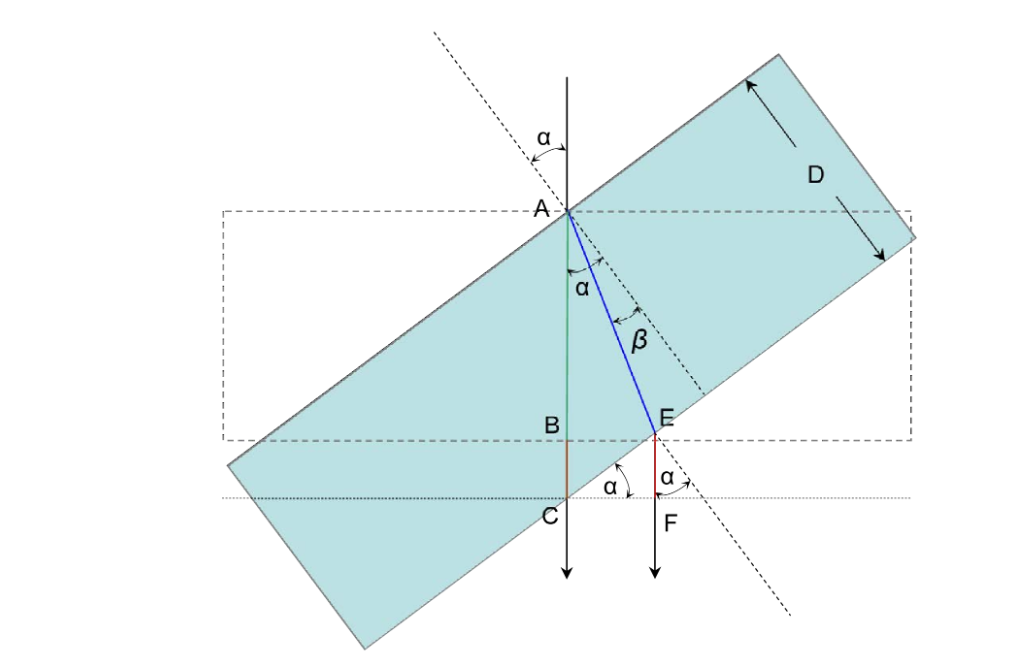
\includegraphics[width=1.0\textwidth]{images/Formula}
		\centering
		\caption{Skizze des Glas in zwei Zuständen: Einfallswinkel $\alpha= 0$ (gestrichelter Quader) und $\alpha>0$ (ausgefüllter Quader).\cite{GlasFormula}} %TODO gestrichelt fine? Quader/Quadrat %TODO cite right?
		\label{fig_glass_rotation}
		\centering
	\end{figure}

	Da sich das Glas in einem Arm des Michelson-Interferometers befindet, durchlaufen Strahlen dieses doppelt.
	Außerdem muss der Gangunterscheid $\Delta$ ein vielfaches der Wellenlänge sein. Der Gangunterschied ist die Differenz der optischen Weglängen:
	\begin{equation}
		\Delta = m\lambda = 2 \cdot \left(\int_{\text{Weg} A \rightarrow F} \! n(s) \, \mathrm{d}s - \int_{\text{Weg} A \rightarrow C} \! n(s) \, \mathrm{d}s \right)
	\end{equation}
	Aus der Geometrie und den konstanten Brechungsindizes folgt
	\begin{equation}
		m\lambda = 2(n\cdot \overline{AE} + \overline{EF} - n \cdot \overline{AB} - \overline{BC}),
		\label{eq_glas_2}
	\end{equation}
	wobei $n$ der Brechungsindex des Glas ist und $n_\text{Luft}=1$ angenommen wird.

	Unmittelbar aus \cref{fig_glass_rotation} zu entnehmen sind
		$\overline{AB} = D$,
		$\overline{AE} = \frac{D}{\cos{\beta}}$,
		$\overline{AC} = \frac{D}{\cos{\alpha}}$,
		$\overline{BC} = \overline{AC} -D = \frac{D}{\cos{\alpha}}-D$,
		$\overline{EF} = \overline{CE} \cdot \sin{\alpha} = D\cdot (\tan{\alpha}-\tan{\beta})\cdot \sin{\alpha}$.
	Ersetzt man die Strecken und dividiert durch $2D$ in \cref{eq_glas_2} folgt:
	\begin{equation}
		\frac{m\lambda}{2D} = \frac{n}{\cos{\beta}} + \sin{\alpha}\tan{\alpha} - \sin{\alpha}\tan{\beta}-n  - \frac{1}{cos{\alpha}} +1
	\end{equation}
	Durch das Snelliusssche Brechungsgesetz $n \cdot \sin{\beta} = \sin{\alpha}$  ergibt sich mit $\cos{\beta}=\sqrt{1-\frac{\sin^2{\alpha}}{n^2}}$:
	\begin{equation}
		\frac{m\lambda}{2D} = \sqrt{n^2-\sin^2{\alpha}} -\cos{\alpha} - n + 1
	\end{equation}
	und quadriert
	\begin{equation}
		\left(\frac{m\lambda}{2D}+ \cos{\alpha}-1+n\right)^2 = n^2-\sin^2{\alpha}
	\end{equation}
	Nach Ausmultiplizieren und Umformen ergibt sich:
	\begin{equation}
		n=\frac{\sin^2{\alpha}+\left(\frac{m\lambda}{2D} + \cos{\alpha}-1\right)^2}{2(1-cos{\alpha}-\frac{m\lambda}{2D})}
	\end{equation}
	Mit $\alpha=\Phi$, und $D=t$ lässt sich dies in die Formel aus der Einführung umstellen:
	\begin{equation}
		n= \frac{(2t-m\lambda)(1-\cos{\Phi})+ \frac{m^2\lambda^2}{4t}}{2t(1-\cos{\Phi})-m\lambda}
	\end{equation}

	\section{Methoden}
	% Bilder von der Website klauen
	% einer will Präsens
	%TODO Glas Nullwinkel per Auge

	\section{Ergebnisse und Diskussion}
	%TODO Unsicherheiten


	\subsection{Beobachtung und Datenanalyse}
	% Allgemeine Beobachtungen
	% Einflüsse von veränderten Parametern auf Messung
	\subsubsection{Unsicherheiten}
	% Berechung nach Aufgabenstellung

	\subsection{Diskussion}
	% Bezug/Nutzen oder sonst was
	% auch hier die Hypothese wiederholen
	% keine Messwerte hier, nach manchen Menschen, zumindest "direkt" erstellte Diagramme net hier, auch wenn Lesbarkeit-bla

	\section{Schlussfolgerung}
	% Rückgriff auf Hypothese und drittes Nennen dieser

	% Quellen zitieren, Websiten mit Zugriffsdatum
	% Verweise auf das Laborbuch (sind erlaubt)
	% Tabelle + Bilder mit Beschriftung
	\printbibliography
\end{document}
